\documentclass{acm_proc_article-sp}

\usepackage{amsmath}
\usepackage{verbatim}
\usepackage{textcomp}
\usepackage{graphicx}
\usepackage{subcaption}
\usepackage{url}
\usepackage{multicol}
\usepackage{tikz}
\usetikzlibrary{positioning}
\usepackage{wasysym}
\usepackage{mathtools}
\DeclarePairedDelimiter{\abs}{\lvert}{\rvert}


\begin{document}

\title{Montreal Real Estate Pricing \\
{\normalsize Code available at: \url{https://github.com/mike-n-7/ML4}}} 
\subtitle{}

\numberofauthors{2} 
\author{
% 1st. author
\alignauthor 
Michael Noseworthy \\
	\affaddr{}
% 2nd. author
\alignauthor Benjamin La Schiazza\\
	\affaddr{260531181}
}

\date{Dec3}

\maketitle
\begin{abstract}
	One of the most important stages most people go through at one point in their lives involves buying or selling a home.  Real estate is the largest asset the average person will ever own and many times functions as not only a shelter but also an investment. The more information parties on either side of the transaction can obtain, the better their decision will be and the chances of losing large sums of money will decrease. While many models have been applied to this market over the years, not many have investigated the role municipal data about infrastructure has on pricing these homes. Through the use of data available through the city of Montreal and a snapshot of the real estate market on the island through select agencies, we look to investigate the impact leveraging municipal data can have on pricing and compare the performance of Linear Regression, Lasso Regression and K nearest neighbours in this setting. Results show that much of the city data played little in the output of the learners used and that poorer performance by the algorithms suggests the truly non-linearity of the problem space.

\end{abstract}

\section{Introduction}

	The real estate market is one of the most important markets in the modern economy because of the nature of the goods exchanged. Shelter is a fundamental need for humans and therefore there is a collective interest in pricing homes correctly. While there are other factors in play, an ill-informed party on either side of the transaction can be burned for non-trivial sums. Any insight into pricing homes properly and consistently would be of great interest all parties involved. 
	
	There have been a number of attempts to model real estate prices using Machine Learning approaches. One of the efforts that was on interest involved pricing Boston suburban homes. [1] The results from this study were very impressive and influenced our choice of features for our data. In this paper, they explored the use of a Linear SVM regression and a partial least squares regression. The former yielded a means-squared error (MSE) of \$10,000 while the latter had a MSE of \$25,000. The interesting point however from their paper is their feature set which included distance to radial highways, density of non-retail businesses in the area as well as local crime rate. These results assured us that decent results have been achieved with the above model of real estate in a comparable city and serve as a benchmark for the results that follow. 
	
	The goal of this project was to attempt to model Montreal homes in it's various boroughs while using open-data from the city of Montreal. [2] Not wanting to simply repeat results that have been obtained before, and ultimately constrained by the data sets at our disposal, we opted to explore the use of different characteristics in describing and modelling homes in the city. We hope to investigate the role of other municipal infrastructure in determining the value of homes and in doing so, convince policy makers that the collection, aggregation and dissemination of municipal/city data can be beneficial to it's residents.


\section{Problem Definition and Description of data}
	
	This project aims to model Montreal housing prices based on a specific set of features in order to determine their importance in marketing a home. As there are all sorts of real estate available on the market, we focused on homes or condos. As alluded to above, we wanted to explore the role that municipal infrastructure has on the prices of homes, something that hasn't been explored in much depth. It is hence a regression task to determine the price of a property.
	
	Our data samples consist of standard descriptions of each property as well as the number of various municipal establishments within 3 KM of the property. This radius was chosen because it represents what we feel is a comfortable walking distance whether it is within the heart of the city or in a suburb. The learning algorithms used include traditional Linear Regression, Lasso Regression and K nearest neighbours (which seemed appropriate!). 

\subsection{Data}

	The real estate market, unlike other traditional markets, does not have a centralized trading "floor" or venue. Parties have the option to deal with an agent or sell the house on their own. As a result price information on available properties isn't centralized. All of the housing data had to be retrieved from brokerage web sites. DuProprio and Royal Lepage web sites were used to get the data needed. They did not offer convenient API's so the sites had to be scrapped for the necessary data. While this provided all the standard descriptors of properties, datasets released by the city of Montreal were needed to locate police stations, family-friendly buildings, handicap friendly buildings as well as numerous other notable infrastructure. Coordinate information for both properties and these entities were used to count instances within a walking radius.
	
	In all 9717 data points were collected. Data points with abnormally high prices (defined in our case as >750000) were removed as they were outliers. As alluded to, the main features were property descriptors (eg. type of property, living area, neighbourhood, latitude, longtitude, number of bathrooms, number of bedrooms etc...) and counts of local municipal infrastructure (eg. fire stations, police stations, monuments, emergency shelters, family quality buildings...). There were [COUNT] features in all and the full list can be found with our code base.
	
\subsection{Missing Data}

	Because our dataset was scraped off of websites, there were a lot of data that were missing. We decided to look at 3 approaches to dealing with missing data, removing those instances altogether, fitting a model to them using Expectation Maximum [3] and predicting values and just filling in with the mean of the collected features. Below is a histogram of the number of data points missing  for various features.
	
	\begin{figure}[h!]
   		\centering
  		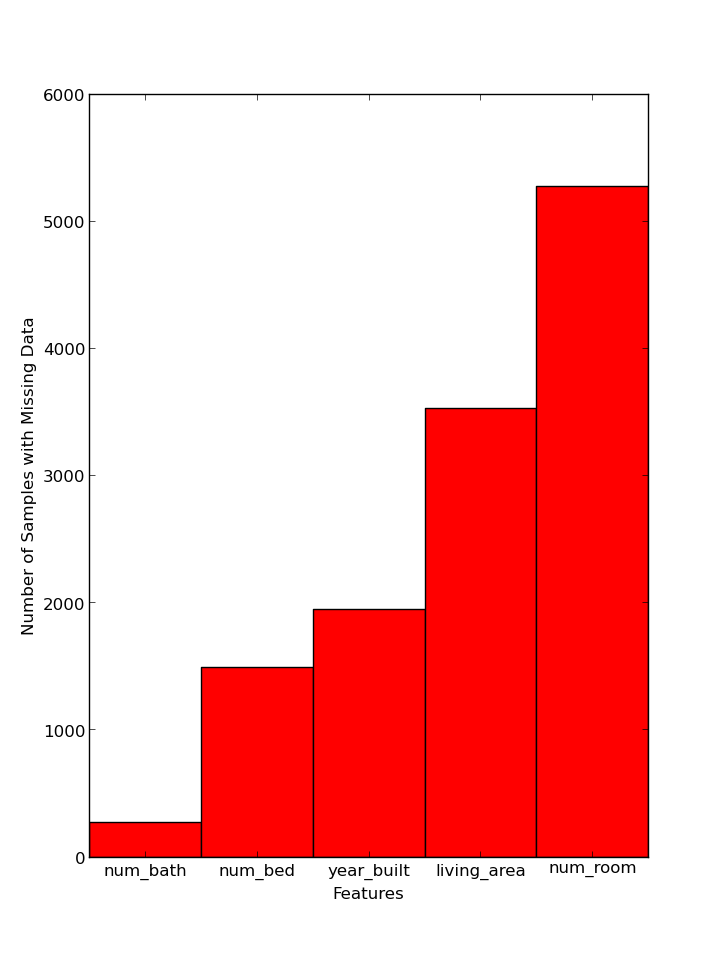
\includegraphics[width=\linewidth]{missing_data.png}
    		\caption{Number of instances with the above features missing. }
    		\label{fig:missingdata}
	\end{figure}
	
\section{Methodology}
	
	Due to the fact that there was a significant amount of missing data, we investigated not only algorithm performance but also methods for treating the missing data. Each algorithm was run on the three datasets resulting from these treatments. Algorithms were optimized for better results on training sets and a held out test set was used for final evaluation.
	
\subsection{Features}
	
	Features consisted of two broad categories, property descriptors and integer counts of the number of instances of municipal infrastructure within walking distance from the datapoint. Many of the features were inherently numerical so they remained untouched. Categorical data such as the property type (house, condo etc...) or the year it was sold (2002-unsold) could have been encoded using integer codes. Research has shown however that one-hot encoding yields better results. [4] These two characteristics hence exploded into a set of binary features.
	
\subsection{Algorithm Selection}
	Below is a brief description of the algorithms considered. They were chosen from a wider set of algorithms because during initial smoke testing they had the best results and showed promise.
	
\subsubsection{Linear Regression}
	Linear Regression is a simple and classic method that fits a line/plane through the data in the space of features. It's hypothesis for a feature space with m features is of the form, \\
	\[  f_{w}(x) = w_{0}  + \sum_{j=1:m}w_{j}x_{j} \] \\

	The w's are the weights that need to be solved for. Different approaches exist for picking these weights optimally. The scikit-learn implementation uses least-squares which seeks to choose a weight vector to minimize,
	\[ Err(w)  = \sum_{i=1:n}(y_{i} - w^{T}x_{i})^{2}\] \\
	
	A closed form solution does exist but the remaining details, while interesting, are not pertinent.
	
\subsubsection{Lasso Regression}
	Lasso Regression is similar in nature to Linear Regression but makes a number of improvements. It is a form of \emph{regularization} which aims to impose constraints on a solution to prevent overfitting. In Lasso Regression, the weights are constrained by penalizing by their absolute value. This forces less important features to have weights of 0 and implicitly weeds out useless features in the process. Because the real estate domain is a bit foreign to us, we simply included features we felt might have influence on property price. This algorithm will help trim them down to a relevant subset.
	
	It solves for a weight vector s.t. \\
	\[ w^{lasso} = argmin_{w}(\sum_{i=1:n}(y_{i} - w_{0} - \sum_{j=1:m}x_{ij}w_{j})^{2} + \lambda\sum_{j=1:m}\abs{w_{j}}) \]
	
	
\subsubsection{K Nearest Neighbours}
	K nearest neighbours take a different approach. The core assumption made with this method is that examples with similar feature values should have similar outputs. Neighbours of a queried datapoint should be used to determine it's value and not points that are far away. In a regression task, once the neighbours have been located, the mean of their values (or a weighted average) is taken to assign to the queried point.
	
	The scikit-learn implementation takes a basic average of the neighbouring data to predict new values. This method is very intuitive but performance really can depend on the nature of the dataset involved. In our case it seems like a very good option because homes tend to be priced similarly to homes in the same (literal) neighbourhood. Beyond the fact that the algorithms name seems apt, it should be able to capture this assumption regarding real estate as literal neighbours will have similar construction dates, sizes and proximity to infrastructure.

\subsection{Implementation Details}
	Raw data had to be scraped from real estate websites. To do so we used the popular Scrapy framework available for python [6]. A spider was written for each website and data from which was loaded through a script into a cohesive raw dataset. This raw data was then cleansed by removing outliers and bad data and extended using the Montreal datasets as discussed previously. All scripts for collecting and pre-processing of data is available in the code base (though Scrapy will need to be installed in order to scrape raw data).
	
	All the algorithms used were implemented in the scikit-learn library. [5] It provides efficient implementations of many useful algorithms and procedures and therefore we wanted to take advantage of the fact that it is available for use. Beyond the implementations of the regression algorithms, it was also used to set up our K sets for our K-Fold cross-validation procedure. 

\subsection{Training/Testing}


\section{Results}
	 The results were generally a bit disappointing when compared to the benchmark paper referenced in the Introduction [1]. Analysis however offers many plausible reasons for this as well as interesting insights. 
	 
\subsection{Linear Regression}
	Below compares the performance of Linear Regression over the three datasets representing approaches to handling missing data. Best performance was with the malformed data removed and yielded a MSE of about \$45,000.
	 
	 \begin{figure}[H]
   		\centering
  		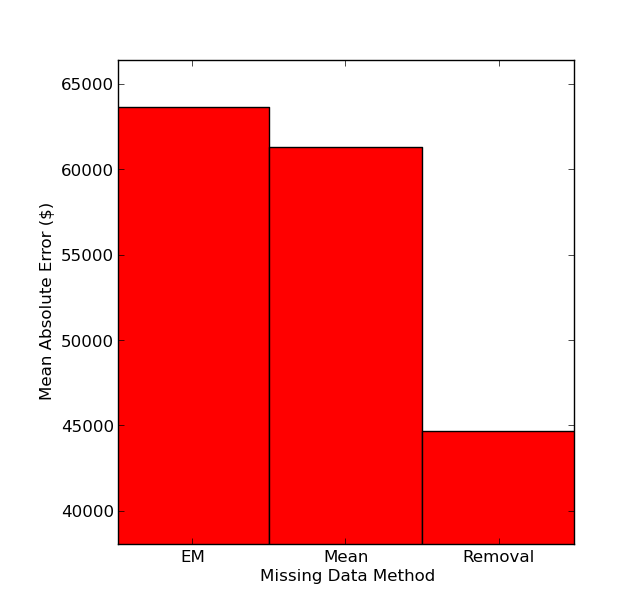
\includegraphics[width=\linewidth]{linear_regression_tuning.png}
    		\caption{Performance of Linear Regression algorithm}
    		\label{fig:linreg}
	\end{figure}
	
\subsection{Lasso Regression}
	Lasso's lambda parameter was optimized but performance seemed to be only marginally affected. Figure 3 shows once again that removing the missing data was most fruitful. Best MSE was approximately \$44,000.
	
	 \begin{figure}[H]
   		\centering
  		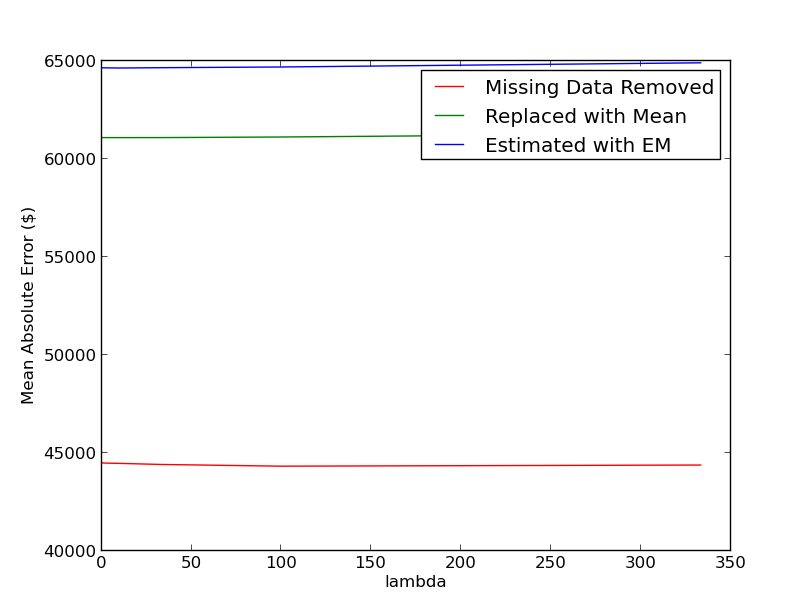
\includegraphics[width=\linewidth]{lasso_tuning_plot.png}
    		\caption{Performance of Lasso Regression algorithm}
    		\label{fig:lassoreg}
	\end{figure}
	
\subsection{K Nearest Neighbours}
	The optimal K was [INSERT], as shown below. Once again simply removing the bad data yielded the best results. 
	
	\begin{figure}[H]
   		\centering
  		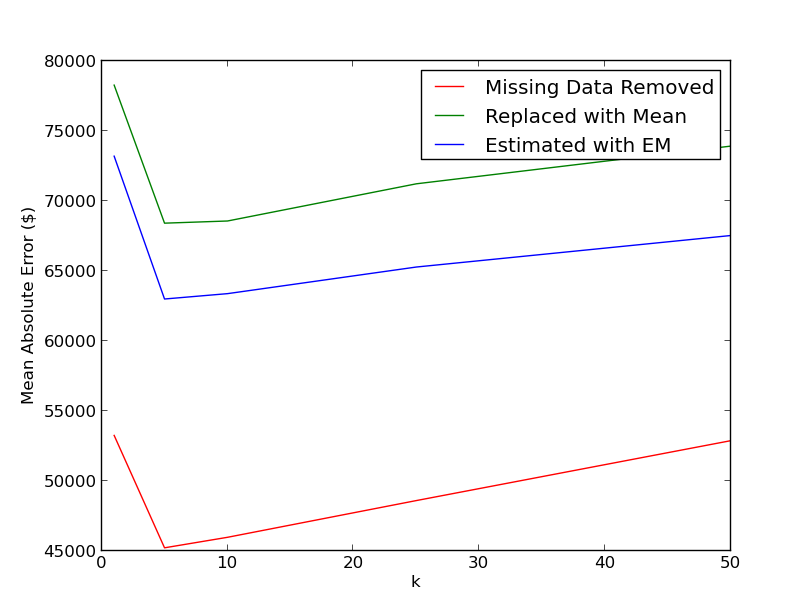
\includegraphics[width=\linewidth]{knn_tuning.png}
    		\caption{Performance of K-Nearest Neighbours as a function of K}
    		\label{fig:knn}
	\end{figure}


\section{Discussion}

\end{document}
